\subsection{Category Classifier}
\label{sec:category}

The {\em Category method} allows the user to separate the training data (and accordingly the 
application data) into disjoint sub-populations exhibiting  different
properties. The separation into phase space regions is done by applying requirements
on the input and/or {\em spectator} variables (variables defined as spectators are 
not used as direct inputs to MVA methods). 
It thus reaches beyond a simple sub-classification of the original feature space.
In each of these disjoint regions (each event must belong to one and only one region), 
an independent training is performed using the most appropriate MVA method, training 
options and set of training variables in that zone. The division into categories in 
presence of distinct sub-populations reduces the correlations between the training 
variables, improves the modelling, and hence increases the classification and 
regression performance.\footnote
{
   This is particularly the case for projective likelihood methods, even when 
   including prior decorrelation of the input data (\cf\  Sec.~\ref{sec:likelihood}). 
}
Another common application is when variables are not available 
in some phase space regions. For example, a sub-detector may only cover a fraction of
the training data sample. By defining two categories the variables provided by this 
detector could be excluded from the training in the phase space region outside 
of its fiducial volume. Finally, an advantage of categorisation, often exploited 
in likelihood fits, also lies in the gain of signal significance when the fraction of 
signal events in the event sample differs between the categories. 

We point out that the explicit use of the Category method is not mandatory. The categorisation
functionality can be achieved by hand by training independent MVAs in each of the 
disjoint regions. Our experience however shows that often the corresponding bookkeeping
is considered too cumbersome and the required categorisation is not performed, 
thus leading to performance loss.\footnote
{
   In the above example with the reduced detector fiducial acceptance, it often occurs that 
   non-physical values (``$-99$'') are assigned to the variables for events where they are 
   not available. Inserting such meaningless (apart from indicating the category) 
   values into an MVA penalises its performance. 
}
The Category method is straightforward to implement and should help in almost all analyses
to better describe the training sample. Performance comparison with the corresponding
non-categorised method should guide the user in his/her choice. 

For the current release, the Category method is only implemented for classification. 
Extension to regression is however straightforward and should follow soon. 

\subsubsection{Booking options}

The Category method is booked via the command:
\begin{codeexample}
\begin{tmvacode}
TMVA::IMethod* category = factory->BookMethod( TMVA::Types::kCategory, 
					       "Category",
					       "<options>" );
\end{tmvacode}
\caption[.]{\codeexampleCaptionSize Booking of the Category method: the first 
		   argument is a predefined enumerator, the second argument is a user-defined 
		   string identifier, and the third argument is the configuration options string.
         Individual options are separated by a ':'. 
         See Sec.~\ref{sec:usingtmva:booking} for more information on the booking.}
\end{codeexample}

The categories and sub-classifiers are defined as follows:
\begin{codeexample}
\begin{tmvacode}
TMVA::MethodCategory* mcategory = dynamic_cast<TMVA::MethodCategory*>(category);
mcategory->AddCategory( "<cut>",
		      "<variables>",
		      TMVA::Types::<enumerator>, 
		      "<sub-classifier name>", 
		      "<sub-classifier options>" );
\end{tmvacode}
\caption[.]{\codeexampleCaptionSize Adding a category to the Category method: 
         the first argument is the cut that defines the category, the second defines
         is the set of variables used to train this sub-classifier, the third argument 
         is the predefined enumerator of the sub-classifier, the fourth argument is a 
         user-defined string identifier of the sub-classifier, and the last argument
         sets the configuration options of the sub-classifier. Individual variables 
         and options are both separated by a ':'. See Sec.~\ref{sec:category:impl} 
         for further information on cuts and variables. The dynamic cast is required
         to allow access to specific Category members. }
\end{codeexample}

There are no options implemented for the Category method itself, apart from those 
common to all methods (\cf\  Option Table~\ref{opt:mva::methodbase} on 
page~\pageref{opt:mva::methodbase}). The available options for the sub-classifiers 
are found in the corresponding sections of this Users Guide.

The following example illustrates how sub-classifiers are added:
\begin{codeexample}
\begin{tmvacode}
mcategory->AddCategory( "abs(eta)<=1.3",
		      "var1:var2:var3:var4:", 
		      TMVA::Types::kFisher,
		      "Category_Fisher",
		      "H:!V:Fisher" );
mcategory->AddCategory( "abs(eta)>1.3",
		      "var1:var2:var3:", 
		      TMVA::Types::kFisher,
		      "Category_Fisher",
		      "H:!V:Fisher" );
\end{tmvacode}
\caption[.]{\codeexampleCaptionSize Adding a category with sub-classifier of type Fisher: 
           the cut in the first argument defines the region to which each of the 
           sub-classifiers are applied, the second argument is the list of variables 
           which are to be considered for this region (in this example {\tt var4} is  
           not available when {\tt abs(eta)>1.3}), the third argument contains
           the internal enumerator for a classifier of type Fisher (the MVA method may
           differ between categories, the fourth
           argument is the user-defined identifier, and the fifth argument 
           contains the options string for the Fisher classifier. The variable {\tt eta}
           must have been defined as an input or spectator variable. }
\end{codeexample}			

\subsubsection{Description and implementation}
\label{sec:category:impl}

The Category method is implemented in an entirely transparent way, conserving full
flexibility for the user on which input variables, MVA method and options to use in 
each category, and how the category should be defined. 

The categories are defined via cuts on the input and/or spectator variables. These 
cuts can be arbitrary boolean expressions or may involve any number of variables. 
In case of particularly intricate category definitions it may turn out advantageous 
for the user to pre-define and pre-fill category variables, and use those as spectators 
in TMVA to set an event's category. It is required that the cuts are defined in such 
a way that they create disjoint event samples. TMVA will issue a fatal error in case 
of an ambiguous category definition. 

The variables used for the training of each of the sub-classifiers can be chosen from 
the variables and spectators that have been defined in the TMVA script. The 
individual variables have to be separated by a ':'. The distinction between input 
variables and spectators is necessary to allow performance comparisons
between categorised and non-categorised methods within the same training and evaluation 
job (spectator variables would not be used by non-categorised methods). 

The advantage offered by the Category classifier is illustrated with the following 
academic example. We consider four uncorrelated and Gaussian distributed input 
variables for training. The mean values of the variables are shifted between signal 
and background, hence providing classification information. In addition, all mean 
values (signal {\em and} background) depend on a spectator variable \code{eta}: for 
{\tt abs(eta)>1.3} ({\tt abs(eta)<=1.3}) they have a positive (negative) offset. 
Hence, the Gaussians are broader and the variables receive an effective correlation
when integrating over \code{eta}. The distributions for signal and background of 
one out of the four variables is shown for both \code{abs(eta)} categories in 
Fig.~\ref{fig:cat:absetacats}. Figure~\ref{fig:cat:roc} shows the ROC curves
(\cf\  Sec.~\ref{sec:displayingResults}) of the categorised and non-categorised
Fisher and Projective Likelihood classifiers. Optimum performance is recovered 
by the Category classifier. 
\begin{figure}[p]
\begin{center}
  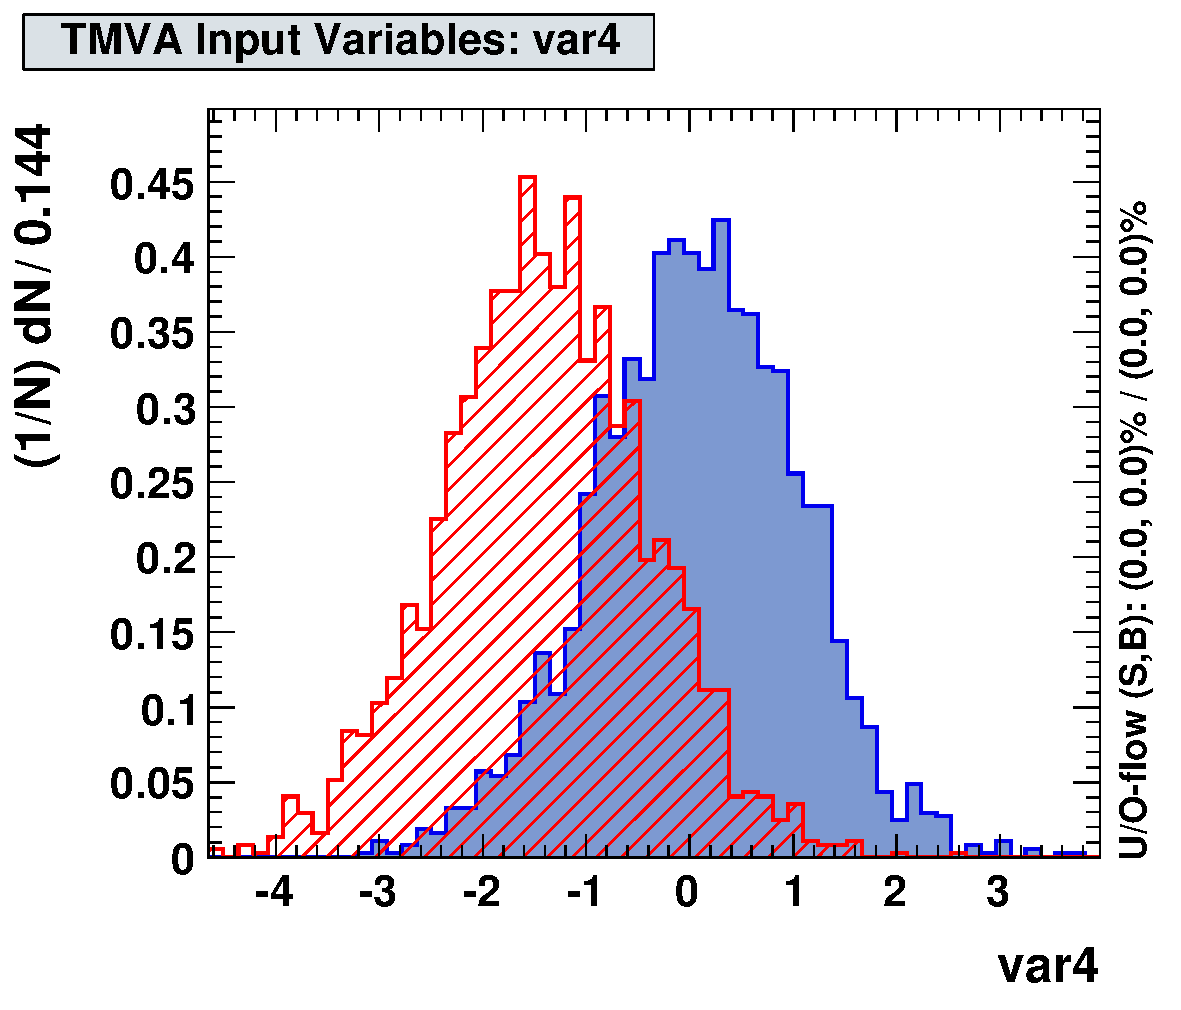
\includegraphics[width=0.49\textwidth]{plots/category_var4_cat1}
  \hspace{-0.0cm}
  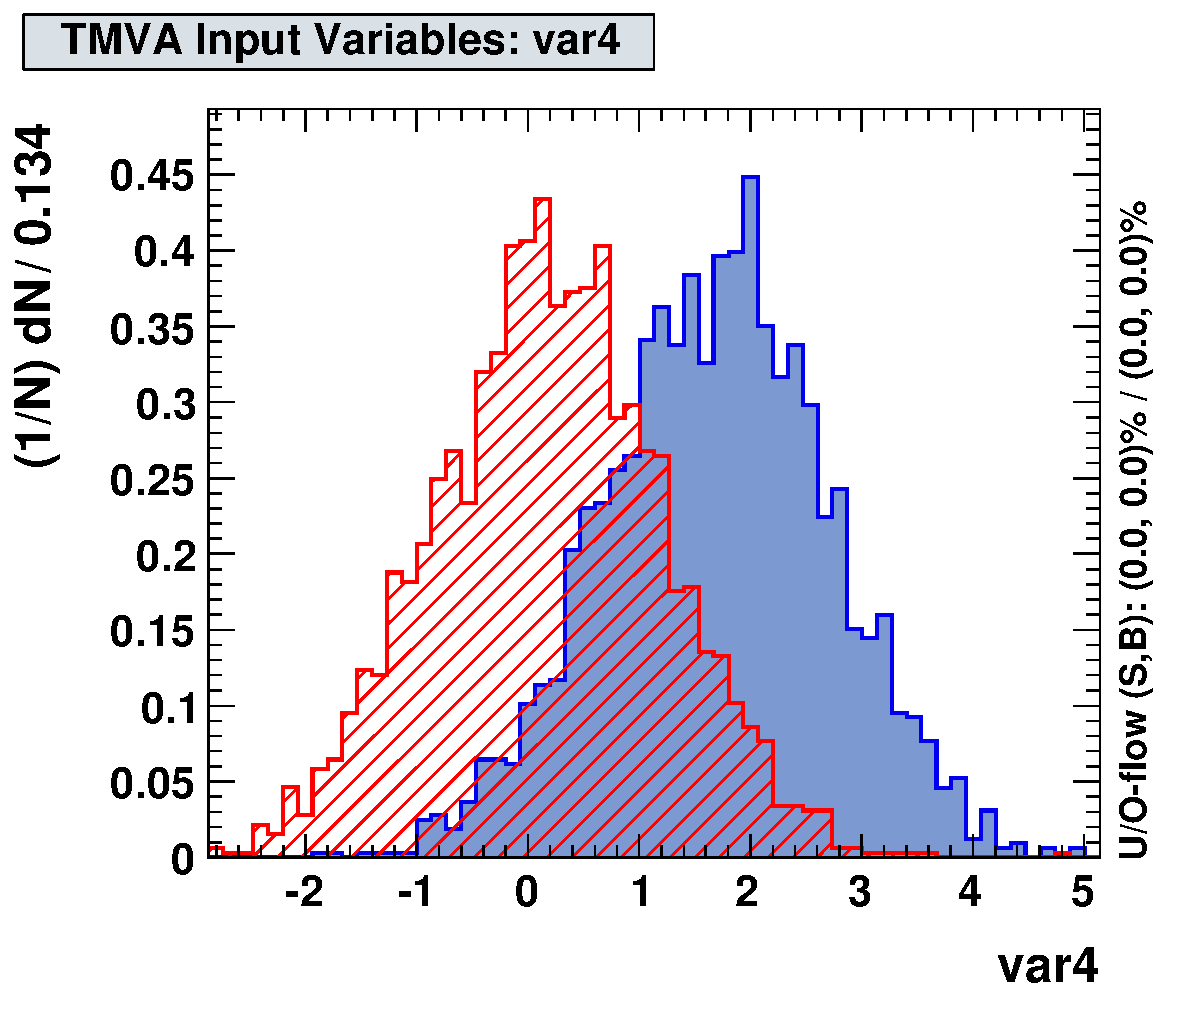
\includegraphics[width=0.49\textwidth]{plots/category_var4_cat2}
\end{center}
\vspace{-0.6cm}
\caption[.]{Examples for the usage of categories. The variable {\tt var4} depends 
            on {\tt abs(eta)}: for {\tt abs(eta)<=1.3} (left plot), the signal and 
            background Gaussian distributions are both shifted to lower values, while 
            for {\tt abs(eta)>1.3} (right plot) shifts to larger values have been applied. 
            Ignoring this dependence, broadens the inclusive Gaussian distributions
            and generates variable correlations (here a coefficient of +$0.4$ between {\tt var3} 
            and {\tt var4}) due to the existence of distinct subsamples. The Category 
            classifier treats the two cases independently, thus recovering optimal 
            separation.}
\label{fig:cat:absetacats}
%\end{figure}
%\begin{figure}[t]
\vspace{0.7cm}
\begin{center}
  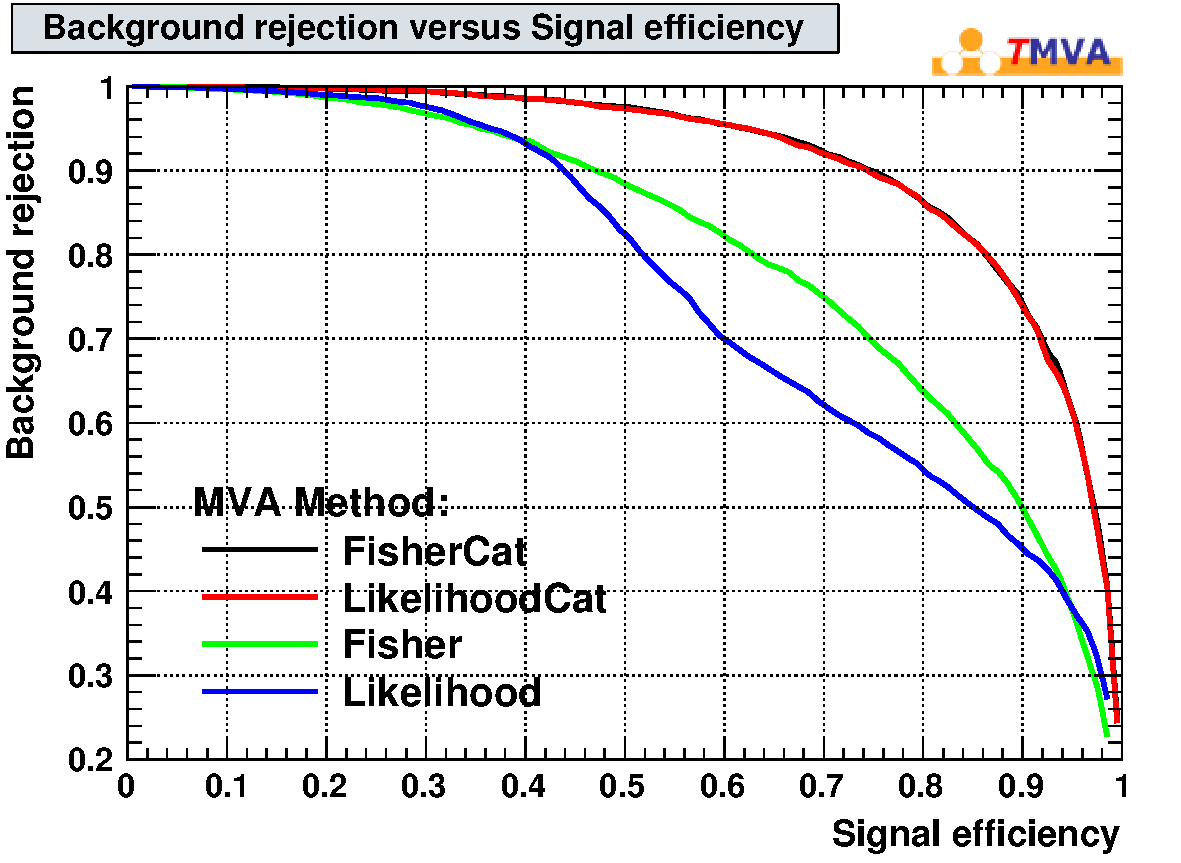
\includegraphics[width=0.65\textwidth]{plots/category_rejBvsS}
\end{center}
\vspace{-0.5cm}
\caption[.]{ROC curves for categorised and non-categorised Fisher and Projective Likelihood
            classifiers applied to an academic four-Gaussian example with {\tt eta}-dependent
            mean values distinguishing two categories (\cf\  Fig.~\ref{fig:cat:absetacats} for the
            category-dependent signal and background distributions of one of the four input 
            variables). The categorised (``...Cat'') classifiers recover optimum performance
            (their red and black curves are superimposed). }
\label{fig:cat:roc}
\end{figure}

\subsubsection{Variable ranking}

Due to the nature of the Category classifier it does not provide a
general variable ranking. As far as available, the sub-classifiers 
will provide ranking for each category.

\subsubsection{Performance}

The performance of the Category method depends entirely on the judicious choice
of the categories, properly separating events with different properties, and on 
the performance of the sub-methods within these categories. Control by performance
comparison with the corresponding non-categorised methods allows to measure the 
performance gain, and to assess whether categorisation improves the classification. 

